% Chapter Template

\chapter{Scaffold} % Main chapter title

\label{Chapter7} % Change X to a consecutive number; for referencing this chapter elsewhere, use \ref{ChapterX}

 %----------------------------------------------------
 
The scaffolds are three-dimensional supports that provide cells with an environment in which adhere, differentiate and multiply. Tissue engineering and scaffolds have been developed with the aim of promoting the regeneration of damaged tissues of the body, to solve the problems related to \emph{autologous grafts} and \emph{donor transplants}. \\ Autologous grafts ( i.e. of skin or bone) require longer surgical time and are more invasive (due to the tissue harvesting from a donor site and the implantation in the damaged site). Furthermore, the tissue in the donor site is not always sufficient to regenerate the damaged tissue. Regards to the homologous grafts (from donor of the same species) the concern is in the scarcity of donors and the biological risk of infection and rejection. \\
To provide the best environment for each group of cells to grown, scaffolds made from a wide variety of materials have been described. Each tissue is in fact unique for mechanical and functional properties, as well as for its micro and macrostructure. \\ The introduction of additive manufacturing techniques in the production of scaffolds has brought novelty in the materials used and combinations of these, and has made possible the exploration of complex designs. The scaffolds can be made of biological polymers, synthetic polymers, ceramic materials and combinations of these \parencites{Reference128}. \\
To promote cell survival, the spread of cells and nutrients and the removal of metabolites and waste products must be facilitated by the scaffold structure. The \emph{porosity} of the scaffold is therefore a fundamental parameter, along with the \emph{porosity interconnection} (that describes how the porosities are connected each other inside the volume's boundary). Growth factors and regulatory proteins of cell adhesion can be integrated into scaffolds, to facilitate cell distribution and regulate it in the case of \emph{multiphase scaffolds} \parencite{Reference129}. The scaffold must also be resorbable, and the rate of resorption must be in accordance with the regeneration rate of the tissue to be repaired; the goal of the scaffolds is indeed to stimulate the complete regeneration of the tissue, with the total resorption of the scaffold in the implant site. \\
Among the most recently used dental scaffolds we find ceramic particles such as \emph{tricalcium phosphate} (TCP, TriCalcium Phosphate), \emph{Hydroxyapatite} (HA) and MTA. These materials are used for bone regeneration, along with the collagen or PTFE membranes used to compartmentalize the regeneration site. The ceramic particles form a porous structure that is held together by the blood clot, promoting the spread of cells and nutrients and stimulating bone production. \\ The chemical composition of these granular materials is similar to that of bone, the high roughness of the surface allows the stabilization of the clot, the adsorption of growth factors and increase cell adhesion. However, the porosity of these materials is not tunable, because it depends on the aggregation that is randomly created during the formation of the blood clot. The resulting clot is also unstable and unsuitable to support mechanical loads during the early consolidation steps \parencite{Reference131}. The rate of resorption of some of these materials is slow and they often stay in the site for a long time. \\
The use of three-dimensional scaffolds has therefore tried to overcome these limitations, trying to provide an optimal solution to these problems and to increase the predictability of the regenerative treatment. The introduction of additive manufacturing has made it possible to have greater control over the scaffold architecture, leading to encouraging results \parencite{Reference136}, \parencite{Reference137}.\\

\begin{figure}[h]
\vspace{-10pt}
	\begin{center}
	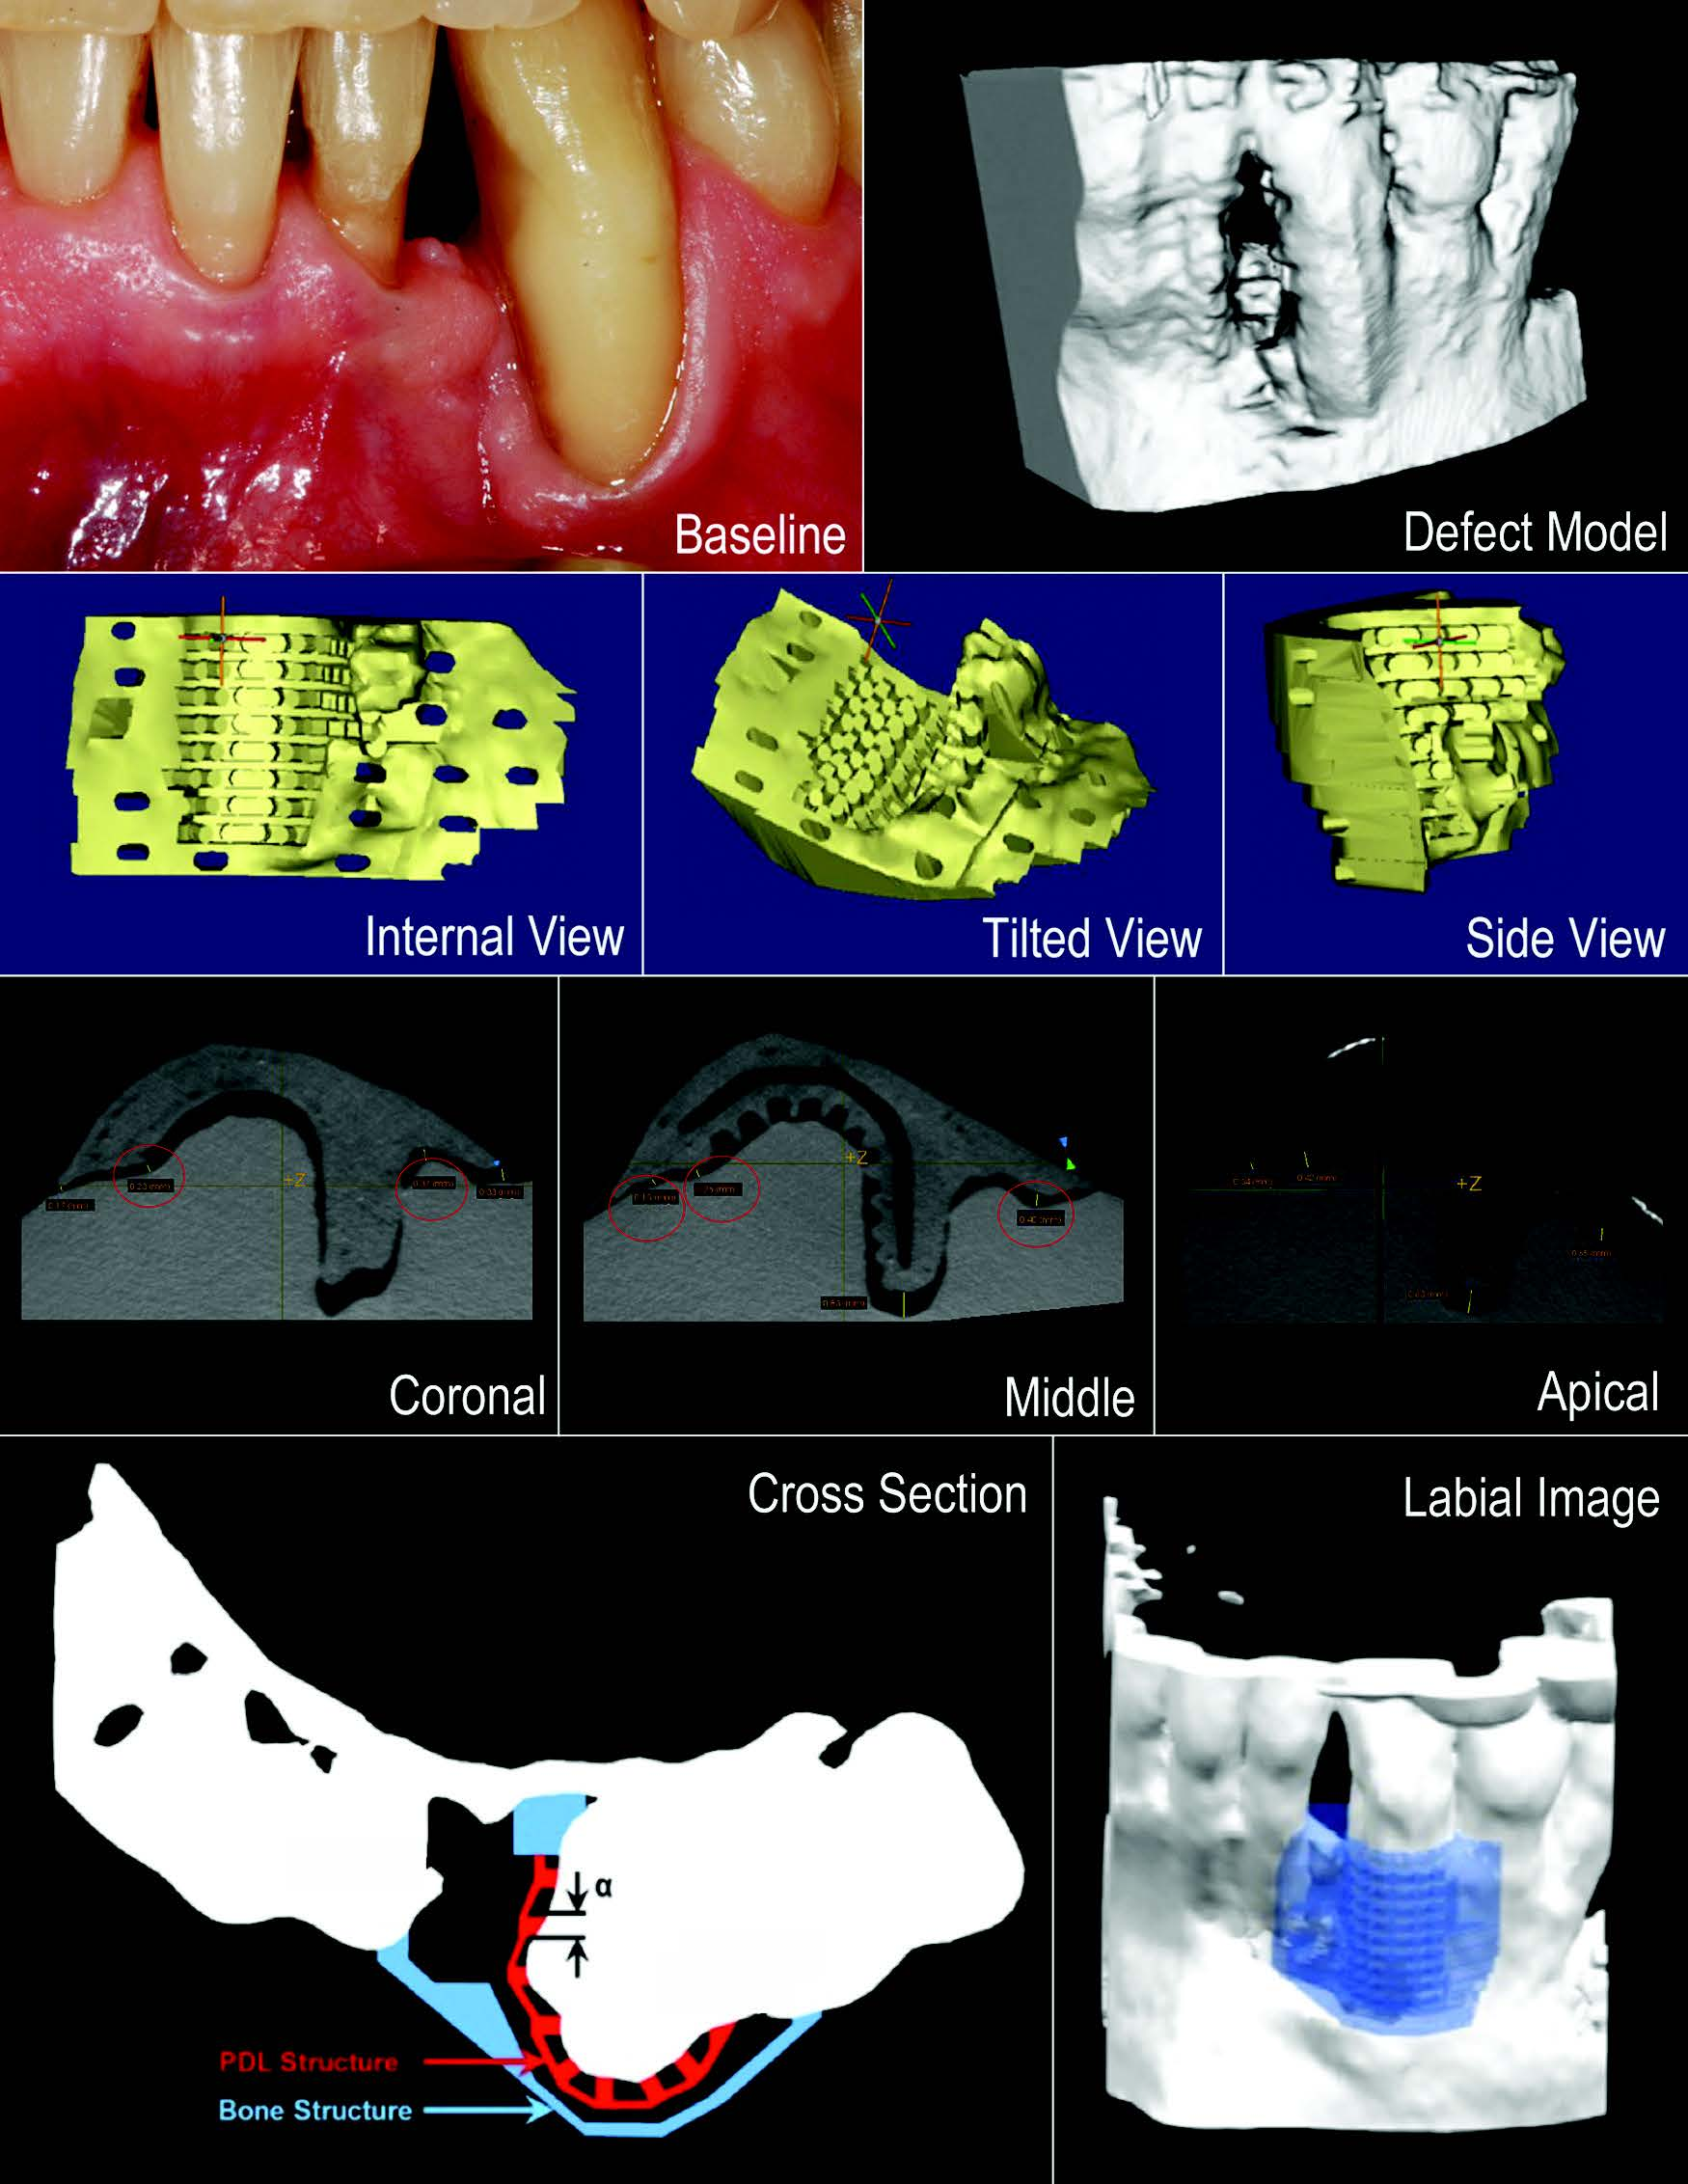
\includegraphics[width=0.6\textwidth, keepaspectratio]{scaf_paro}
    \caption{Scaffold for periodontal regeneration developed by \emph{Rasperini et al} \parencite{Reference134}.}
    \label{fig:scaf_paro}
	\end{center}
\vspace{-20pt}
\end{figure}

Structures in OCT (\emph{octacalcium phosphate}) are \emph{\ textbf {ostoinductive}}, that is, they stimulate the cells already in the damaged site to osteoblastic differentiation \parencite{Reference130}. Osteoinduction is also a property of a composite scaffold made of polycaprolactone and decellularized bone \parencite{Reference132}. A bioactive hydrogel composed of alginate, gelatin and OCT (56, 14, 30 wt\%, respectively) containing Vancomycin or Doxorubicin was tested in order to realize scaffolds with \emph{antibacterial} and \emph{antitumorals} properties, with interesting results \parencite{Reference133}. \\
Lastly, there are promising recent attempts to realize three-dimensional scaffolds for the periodontal ligament regeneration. The periodontal regeneration requires reconstitution of alveolar bone, periodontal ligament and dental cement, so the classic concept of compartmentalization of the periodontal defect has been extended with the use of three-dimensional anisotropic scaffolds, with different compartments and geometric and structural characteristics specific to the tissue to regenerate, such as the guides to direct the regeneration of spatially oriented periodontal fibers. \\
Several authors have made this type of scaffold, and in one case this was tested clinically on the patient; the scaffold was removed after 13 months due to its exposure in the oral cavity \ref{fig:scaf_paro}. The slow resorption of the scaffold material and its reduced porosity have been pointed out to be primarily responsible for the scaffold failure \parencite{Reference134}. \\

\begin{figure}[h!]
 
\begin{subfigure}{0.5\textwidth}
\centering
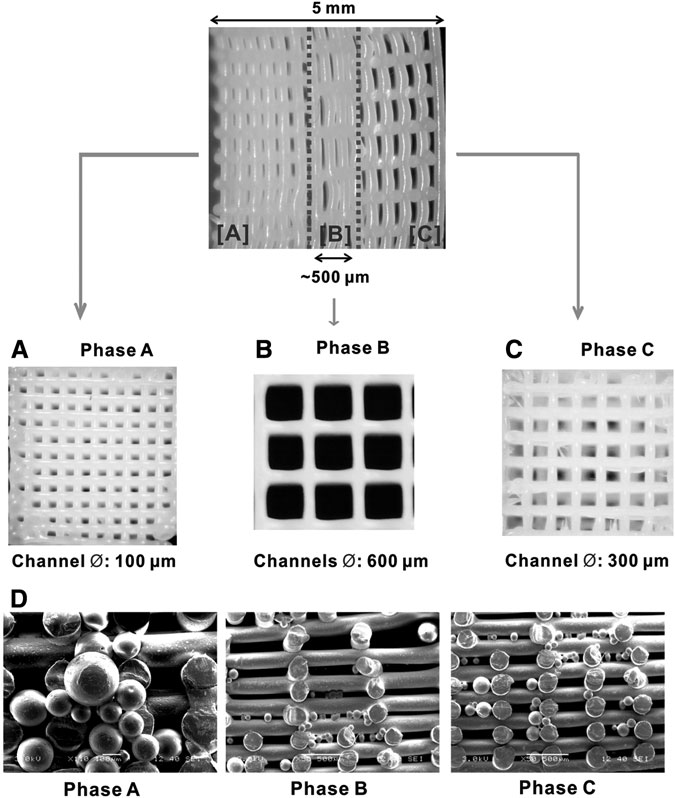
\includegraphics[width=\linewidth, keepaspectratio]{trifase} 
%\caption{}
\label{fig:trifase}
\end{subfigure}
\begin{subfigure}{0.5\textwidth}
\centering
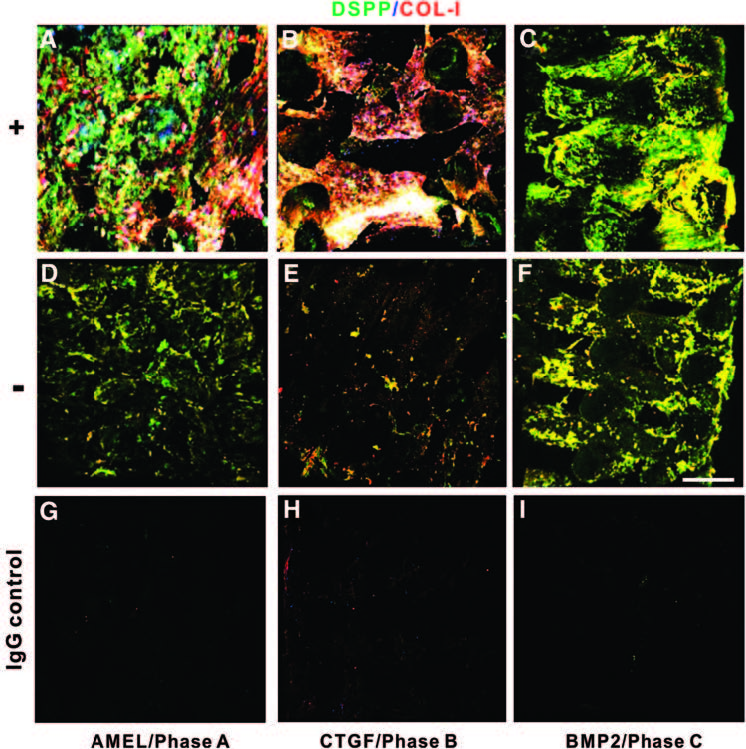
\includegraphics[width=\linewidth, keepaspectratio]{histo}
%\caption{}
\label{fig:histo}
\end{subfigure}
\caption{\textbf{Left}: \emph{triphase scaffold} for periodontal regeneration with growth factors loaded mircrospheres \emph{\textbf{Phase A}}: scaffold for root cement regeneration; \emph{\textbf{Phase B}}: scaffold for periodontal ligament regeneration; \emph{\textbf{Phase C}}: scaffold for alveolar bone regeneration. \textbf{Right}: hystology of the scaffold seeded with DPSC (\emph{Dental Pulp Stem Cell}). \emph{\textbf{First row}} microspheres loaded with growth factors; \emph{\textbf{second row}} empty mocrospheres. DPSC in green (\emph{Dental SialoPhospho Proteine}, stain mineralized regions), \emph{collagen type I} in red, resembling the periodontal ligament. Bar = \SI {200} {\micro\metre}. From \emph{Lee et al} \parencite{Reference135}.}
\label{fig:scaffold_trifase}
\end{figure}
\pagebreak

An interesting design for the regeneration of the periodontal complex was made by Lee \parencite{Reference135}. The author created a PCL-HA structure with differential porosity and enriched it with \emph{microspheres} containing 3 different growth factors, one for each region to be regenerated: \textbf{BMP2} (bone morphogenetic protein 2) for the alveolar bone, \textbf{CTGF} (connective tissue growth factor) for the periodontal ligament and \textbf{Amelogenin} for the root cement \ref{fig:scaffold_trifase}. \\
Then, \emph{dental pulp stem cells} (DPSC) were seeded on the scaffold. The construct thus created was then implanted subcutaneously in guinea pigs and retrieved after 6 weeks. The histology showed the presence of mineralized tissue and oriented and ordered collagen fibers that connect the newly formed cement to the newly formed bone, in an arrangement similar to that of the periodontal ligament (\emph{Sharpey fibers}) \ref{fig:scaffold_trifase}.

\section{Scaffold design}
The design of a scaffold is a compromise between the shape of the defect, the porosity of the scaffold and its mechanical properties, in harmony with the surrounding tissue. This is evident in the realization of scaffolds for the regeneration of bone and cartilage, as the scaffold must provide adequate mechanical properties since its insertion, well before that the injured tissue regenerate. Many designs with various parameters and properties are present in the literature, to underline how each tissue and every functional condition has particular needs to be satisfied during the design phase. \\
Here we describe some basic techniques for the generation of scaffolds which use currently available and open source software. We will not go in deep in the specific features of the scaffold, which have to be adapted according to the field of application.

\subsection{Scaffold design in Cura}
The software we used for slicing our models can easily be used to make simple scaffolds starting from a basic model. Using Cura we will obtain the G-Code of the scaffold, but it will not be possible to obtain a .stl model of the scaffold.

% \ subsubsection {Basic procedure}
To make a scaffold in Cura we have to start from a basic object. We use Blender to create a \textbf{cube} (it is a basic object, found in the main screen in \emph{Add} -> \emph{Mesh} -> \emph{Cube}), export it in .stl format and open it in Cura.
In Cura we can manage the size of the cube from the menu on the left, under \emph{Scale} (you can remove the check in the entry \emph{Uniform Scaling} to resize the object unevenly, for example we can create a parallelepiped starting from the cube). We set the view mode \emph{Layer View} from the top right menu; we will thus see the reconstruction of the G-code. \\
Now let's modify the slicing settings to get a scaffold. The main parameters to be set are the following:

\begin{itemize}

\item In the menù \emph{\textbf{Shell}}:
\begin{itemize}
\item \emph{\textbf{Wall Thickness}}: 0; remove the lateral walls of the model
\item \emph{\textbf{Top/Botton Thickness}}: 0; remove top and bottom of the model
\end{itemize}

\end{itemize}

At this point we will have a model without walls and we will use the infill to manage the parameters of the scaffold \parencite{Reference138}.

\begin{itemize}
\item In the \emph{\textbf{Infill}} menu:

\begin{itemize}
\item \textit{\textbf{Infill Pattern}}: \emph{Lines}; this pattern gives rise to lines deposited in a single direction, which are perpendicular to the lines of the previous layer. This interposition of alternating lines gives rise to a complete interconnection between the pores.\\
\item \emph {\textbf{Infill Line Distance}}: here we can enter a numerical value that will correspond to the distance between consecutive lines in a layer. We use this parameter for the greater control that gives us on geometry compared to Infill Density
\item \emph{\textbf{Infill Line Direction}}: this parameter gives us control over the lines orientation on the XY plane. An angle 0 corresponds to lines parallel to the Y axis, while angle 90 corresponds to lines parallel to the X axis. The angles that we insert will be repeated throughout the height of the object (\textbf{Z axis}). To create layers perpendicular to each other use [0.90].//
We can also create multiple layers in a row with the same angle; for example [0,0,90,90] it will give us two layers parallel to the Y axis and two layers perpendicular to the same axis, which will be repeated until the object is completed. Enter a greater number of consecutive layers oriented in the same way allows the regulation of the pore size on the Z axis; moreover it allows to have a greater interconnection between the pores of the scaffold, making difficult for the melted filament being extruded to close a pore.
\item \emph{\textbf{Gradual Infill Step}}: defines the number of times the infill density increases to the set value, with the least dense area at the beginning and the densest at the end.
\item \emph{\textbf{Gradual Infill Step Height}}: defines the height after which the infill density is doubled, in case of \emph{Gradual Infill Step}.
\end{itemize}

\end{itemize}

The regulation of these parameters allows us to control the geometry of the infill and therefore of the scaffold \ref{fig:mini_cube_full}. The width of each line (\emph{Line Width}) is dependent on the diameter of the nozzle, and is an important parameter to consider during the design. \emph{Brim} or \emph{Raft} can be used to ensure the adhesion of the object to the bed during printing. With the same technique described here it is possible to obtain scaffolds starting from anatomical models \ref{fig:scaffo_mandibola}.
\begin{figure}[t]
\vspace{-10pt}
	\begin{center}
	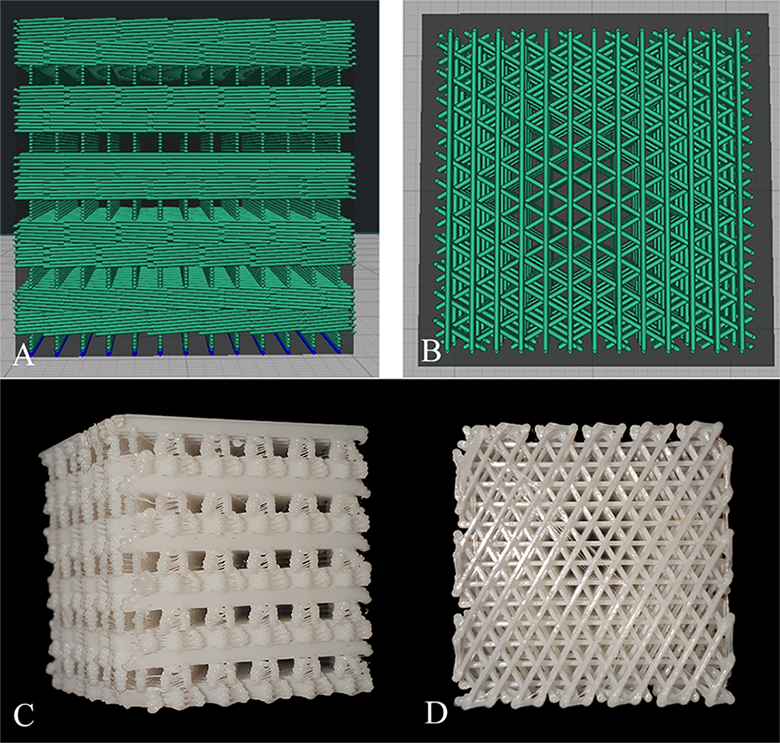
\includegraphics[width=0.9\textwidth, keepaspectratio]{mini_cube_full}
    \caption{\textbf{Scaffold in Cura}, \emph{Layer View}. Cube 20mm per side.
\textbf{A}: front view; \textbf{B}: top view;
\textbf{C} e \textbf{D}: scaffold printed in PLA.
\textbf{Layer Height}: 0.2mm
\textbf{Layer Width}: 0.37mm
\textbf{Nozzle diameter}: 0.4mm
\textbf{Infill Line Directions}: [0,0,0,0,0,0,60,60,60,60,60\-,60,60,120,120,120,120,120,120,120]
\textbf{Line Infill Distances}: \SI{1.52}{\milli\metre}.}
    \label{fig:mini_cube_full}
	\end{center}
\vspace{-20pt}
\end{figure}

\begin{figure}[t]
\vspace{-10pt}
	\begin{center}
	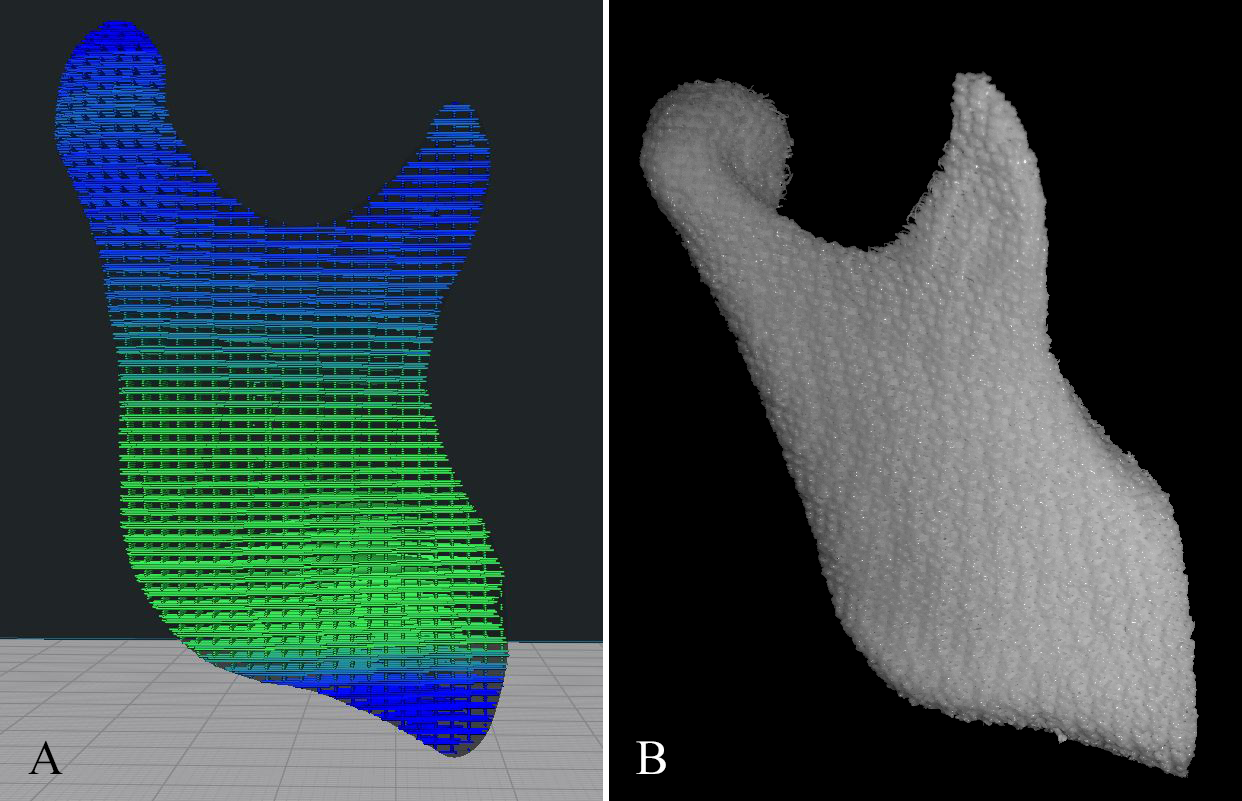
\includegraphics[width=0.9\textwidth, keepaspectratio]{scaffo_mandibola}
    \caption[LoF entry]{Scaffold obtained from a partial model of a mandible.
\textbf{Layer Height}: 0.2mm
\textbf{Layer Width}: 0.37mm
\textbf{Nozzle diametre}: 0.4mm
\textbf{Infill Line Directions}: [0,0,0,90,90,90]
\textbf{Line Infill Distances}: 0.8mm}
    \label{fig:scaffo_mandibola}
	\end{center}
\vspace{-20pt}
\end{figure}

